\chapter{Diseños individuales para la iteración competitiva de Dunia Namour Doughani}
\label{ape:disenyoDunia}

En este apéndice se muestran los diseños individuales realizados por Dunia Namour Doughani para la iteración competitiva. En la Figura \ref{dunia1} se muestra la pantalla de inicio la cual está dividida en 3 secciones, el documento de trabajo, la funcionalidad seleccionada y el PDF cargado. En la Figura \ref{dunia2} se observa la funcionalidad de resumen en la que el usuario pone un texto, pulsa el botón de resumir y le aparece el resumen del texto el cual se puede editar. En cuanto a la Figura \ref{dunia3} se encuentra diseñado el pictotraductor, consta de un campo de texto donde se inserta la frase, al pulsar un botón aparecen los pictogramas. En la Figura \ref{dunia4} se muestra el diseño del ejercicio de flechas que consta de dos columnas, cada una de ellas tiene 2 botones para aumentar o disminuir el número de celdas. En cuanto a la Figura \ref{dunia5} se encuentra representado la funcionalidad de leyenda de colores en la que en un campo de texto se escriben las palabras de la leyenda y a la izquierda de este se encuentra un botón para elegir el color. Finalmente, en la Figura \ref{dunia6} se encuentra diseñado el ejercicio de matemáticas de huecos. En él se elige la longitud de la expresión matemática lo que generará tantos cuadros como longitud se haya puesto y, al pulsar en cada cuadrado aparecerá un desplegable en el que aparecen tanto los números como las operaciones posibles. 

  \begin{figure}[ht!]
    \centering
    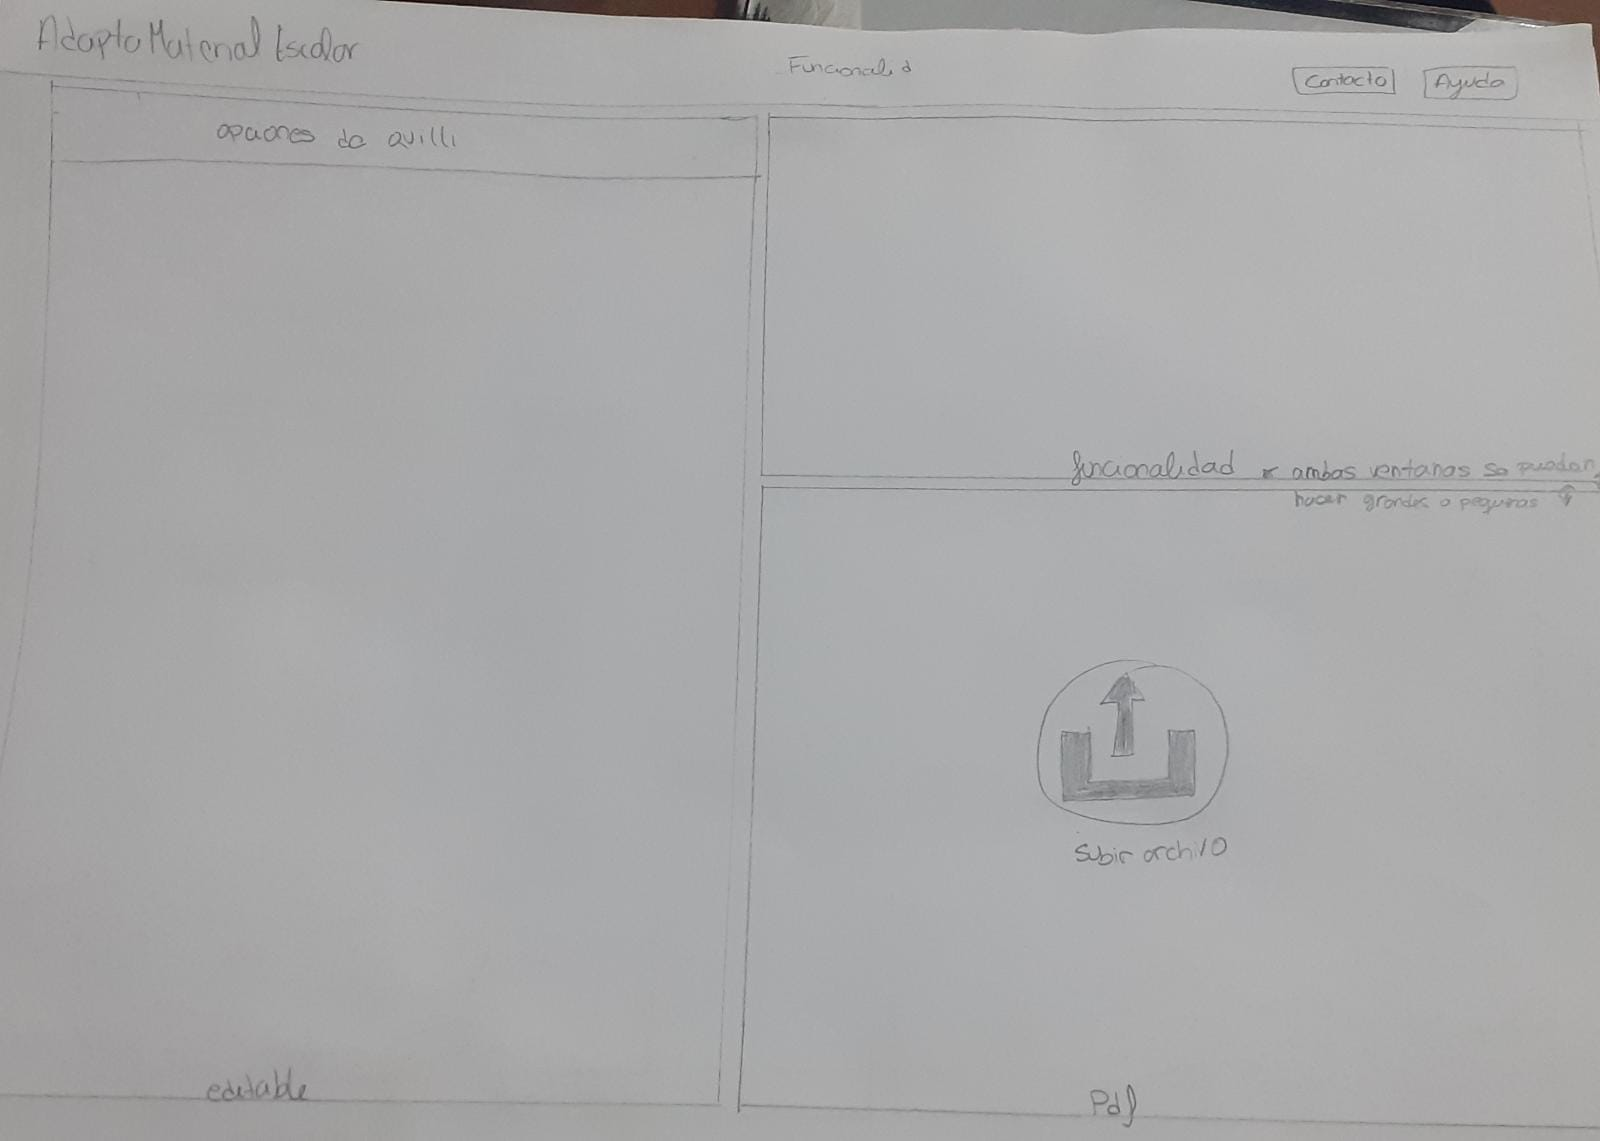
\includegraphics[width=0.6\textwidth]{Diseño/Dunia/principal.jpeg}
    \caption{Diseño pantalla de inicio de Dunia.}
    \label{dunia1}
  \end{figure}

  \begin{figure}[ht!]
    \centering
    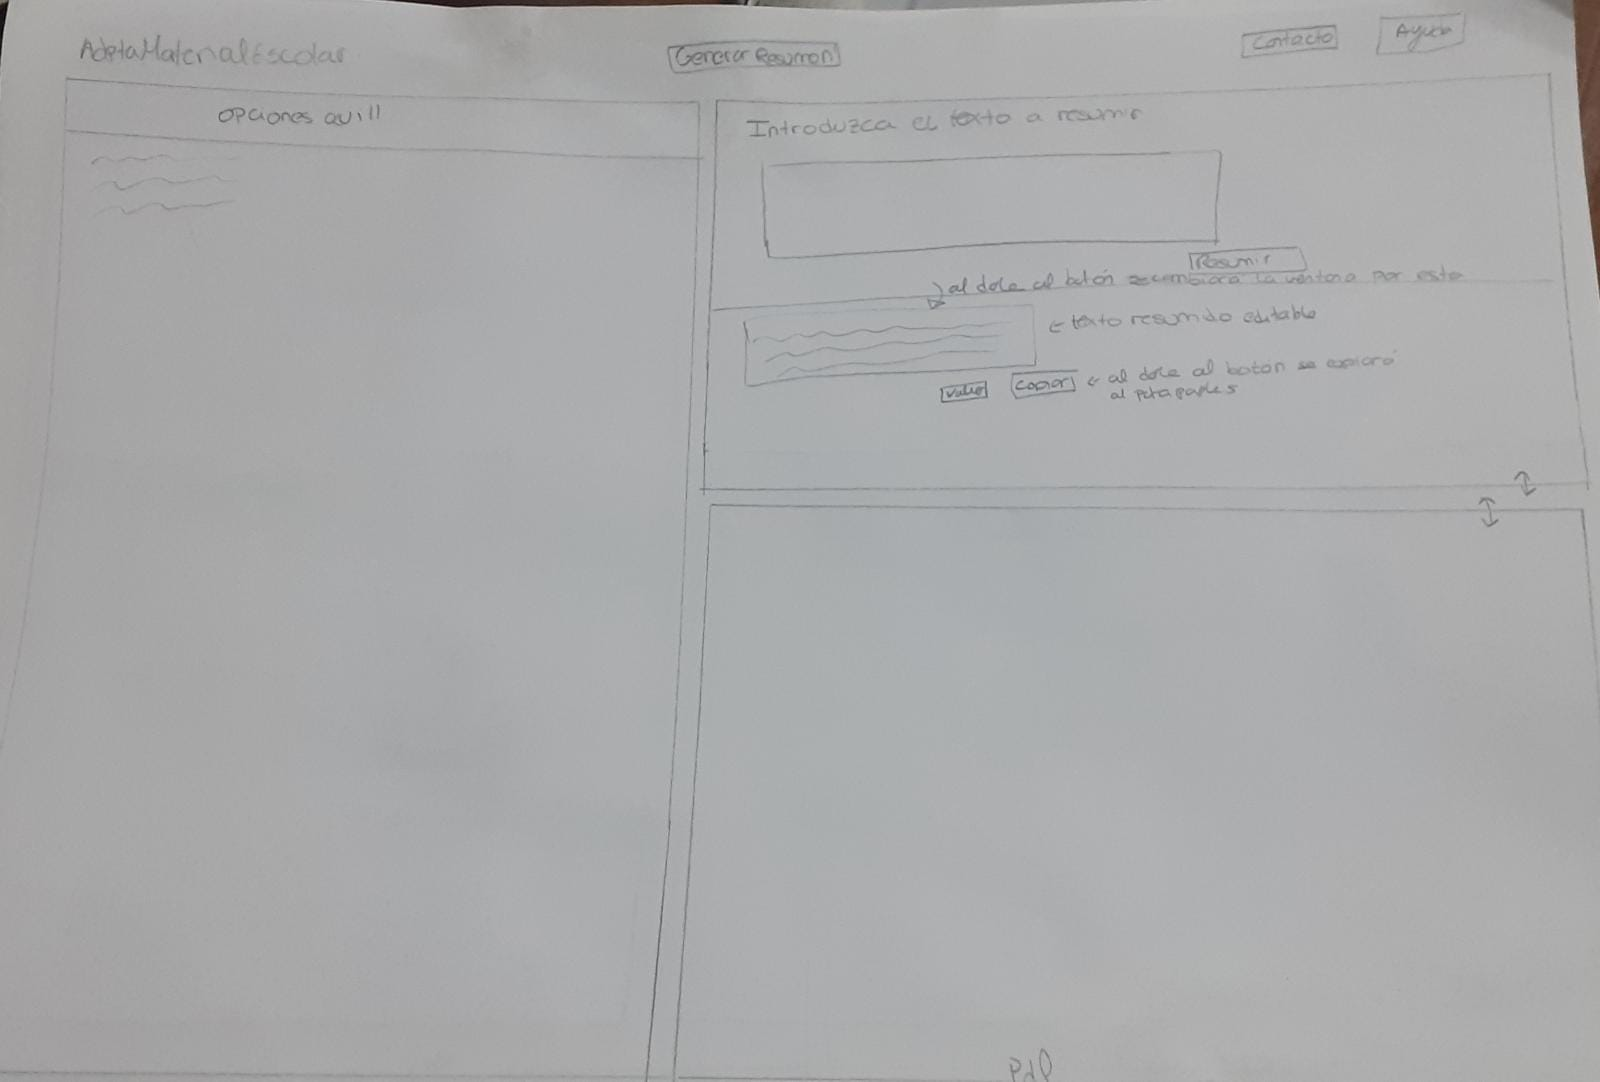
\includegraphics[width=0.6\textwidth]{Diseño/Dunia/resumen.jpeg}
    \caption{Diseño pantalla de generar resumen de Dunia.}
    \label{dunia2}
  \end{figure}

  \begin{figure}[ht!]
    \centering
    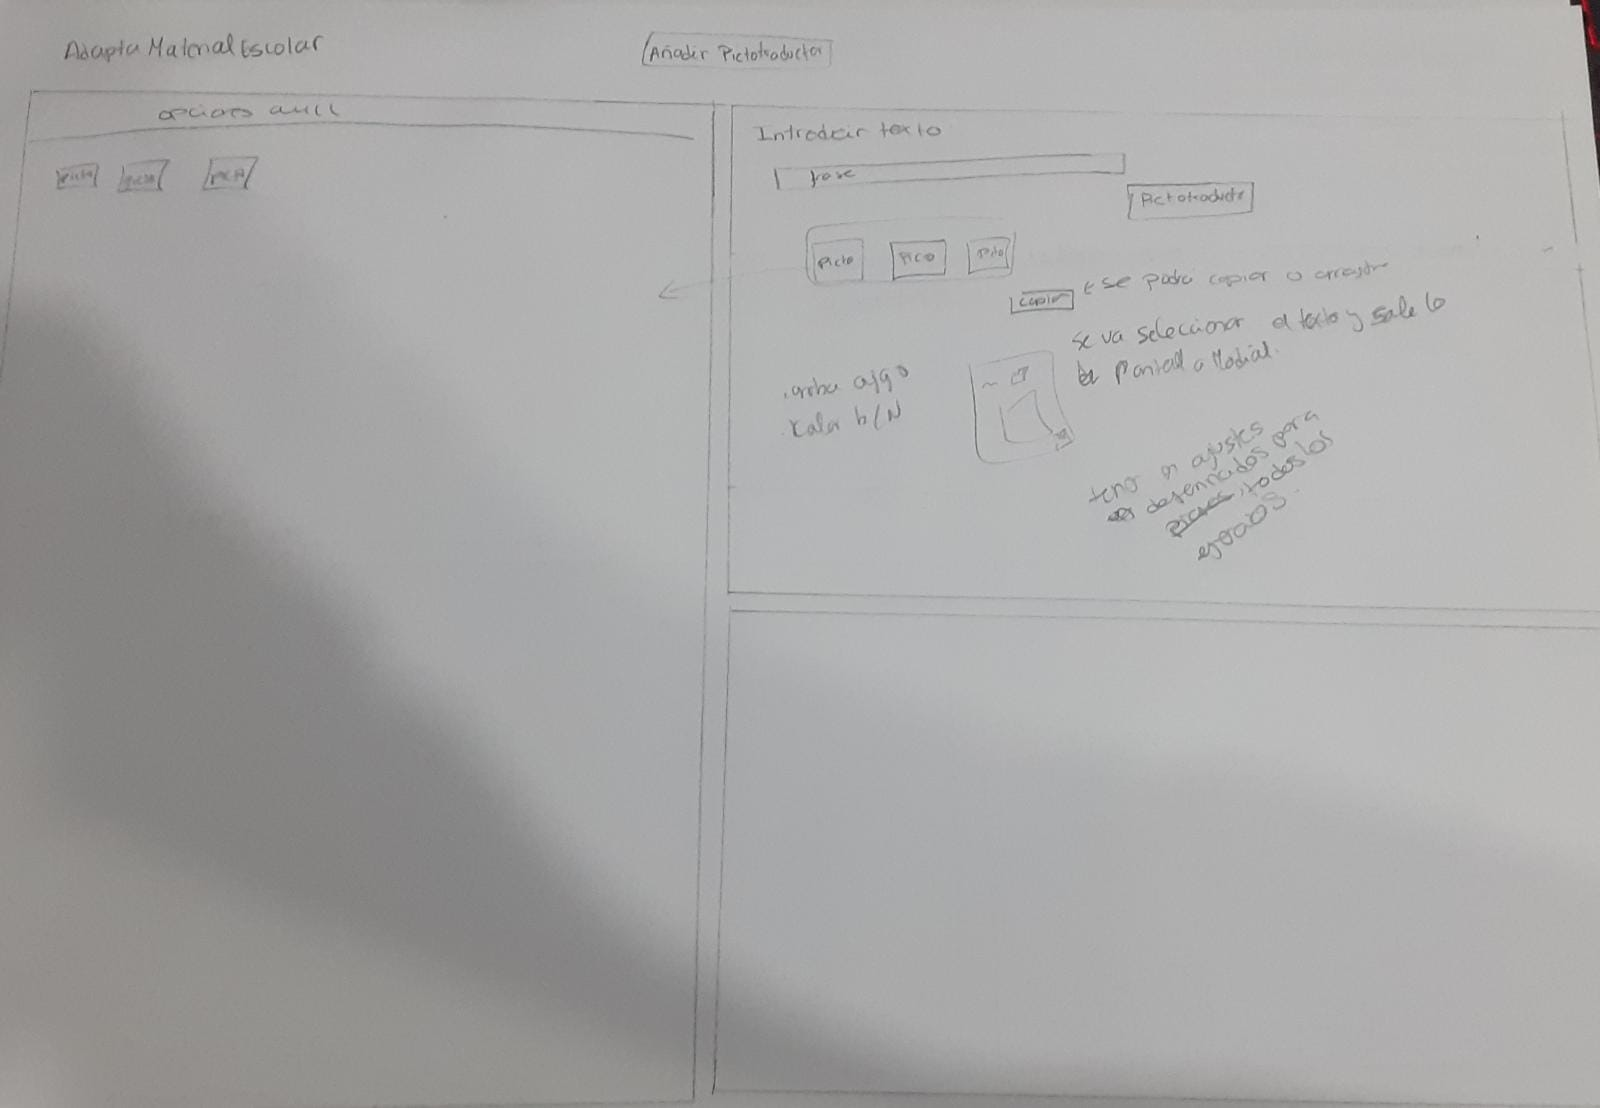
\includegraphics[width=0.6\textwidth]{Diseño/Dunia/picto.jpeg}
    \caption{Diseño de pictotraductor de Dunia.}
    \label{dunia3}
  \end{figure}

  \begin{figure}[ht!]
    \centering
    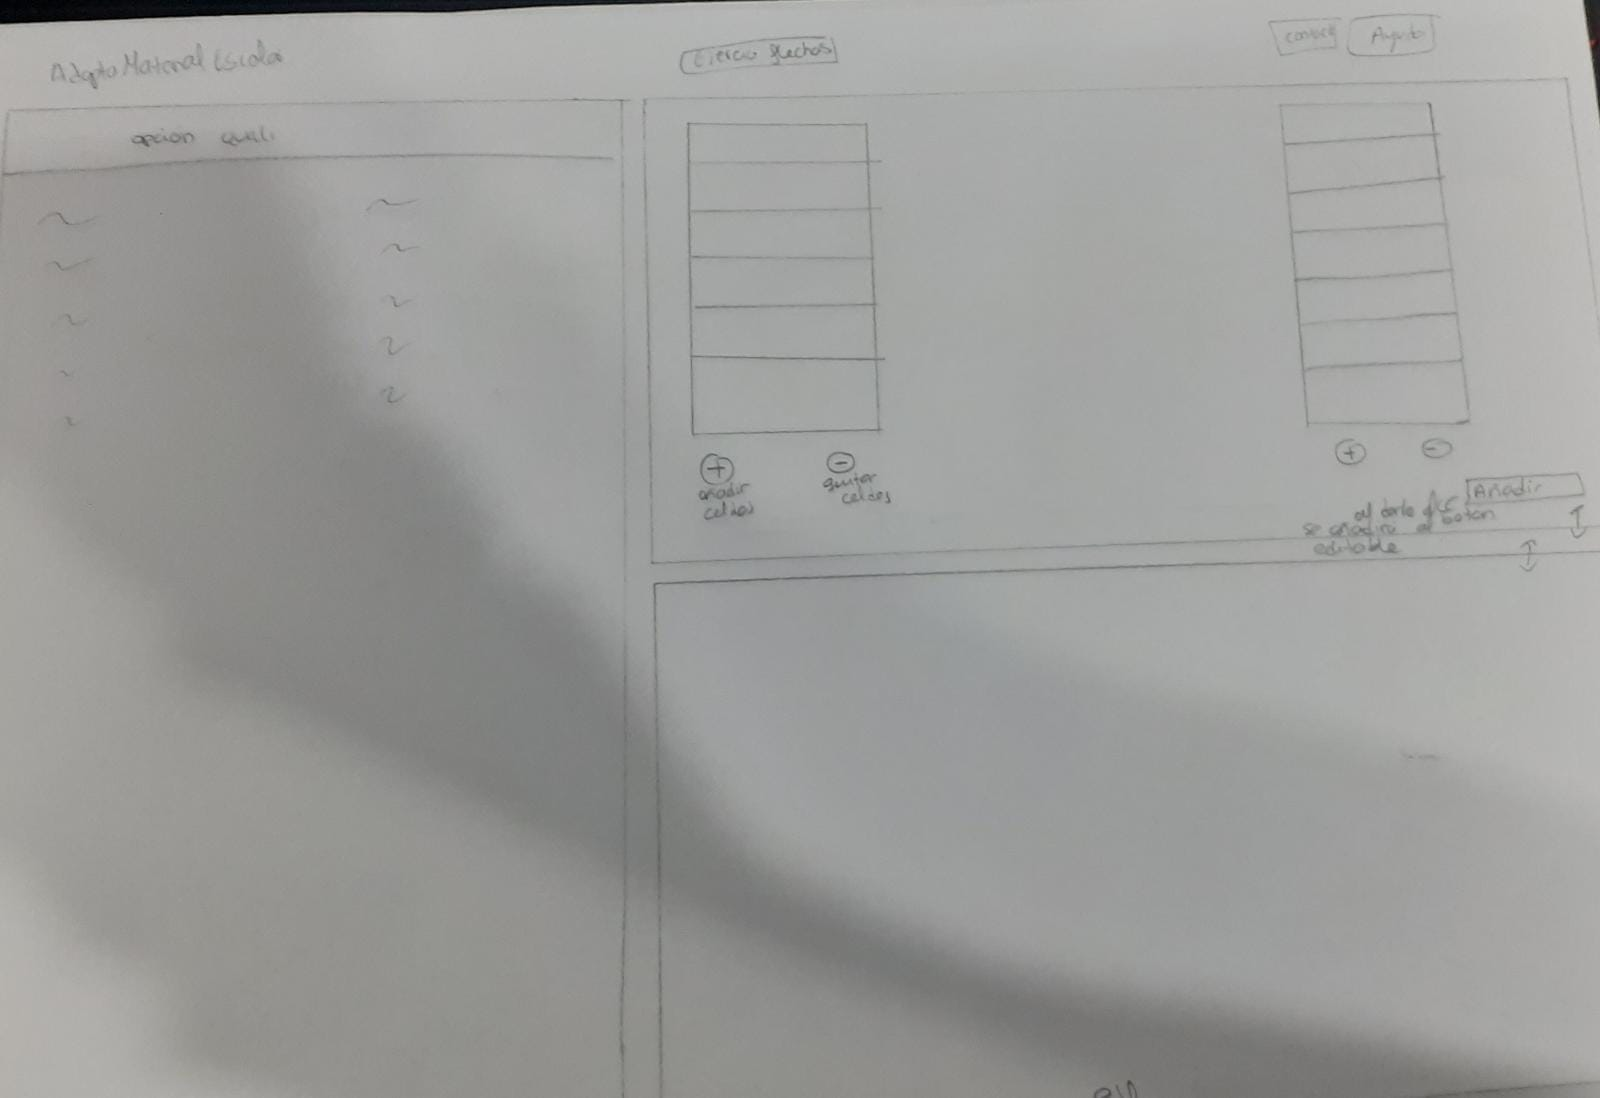
\includegraphics[width=0.7\textwidth]{Diseño/Dunia/flechas.jpeg}
    \caption{Diseño de ejercicios de flechas de Dunia.}
    \label{dunia4}
  \end{figure}

  \begin{figure}[ht!]
    \centering
    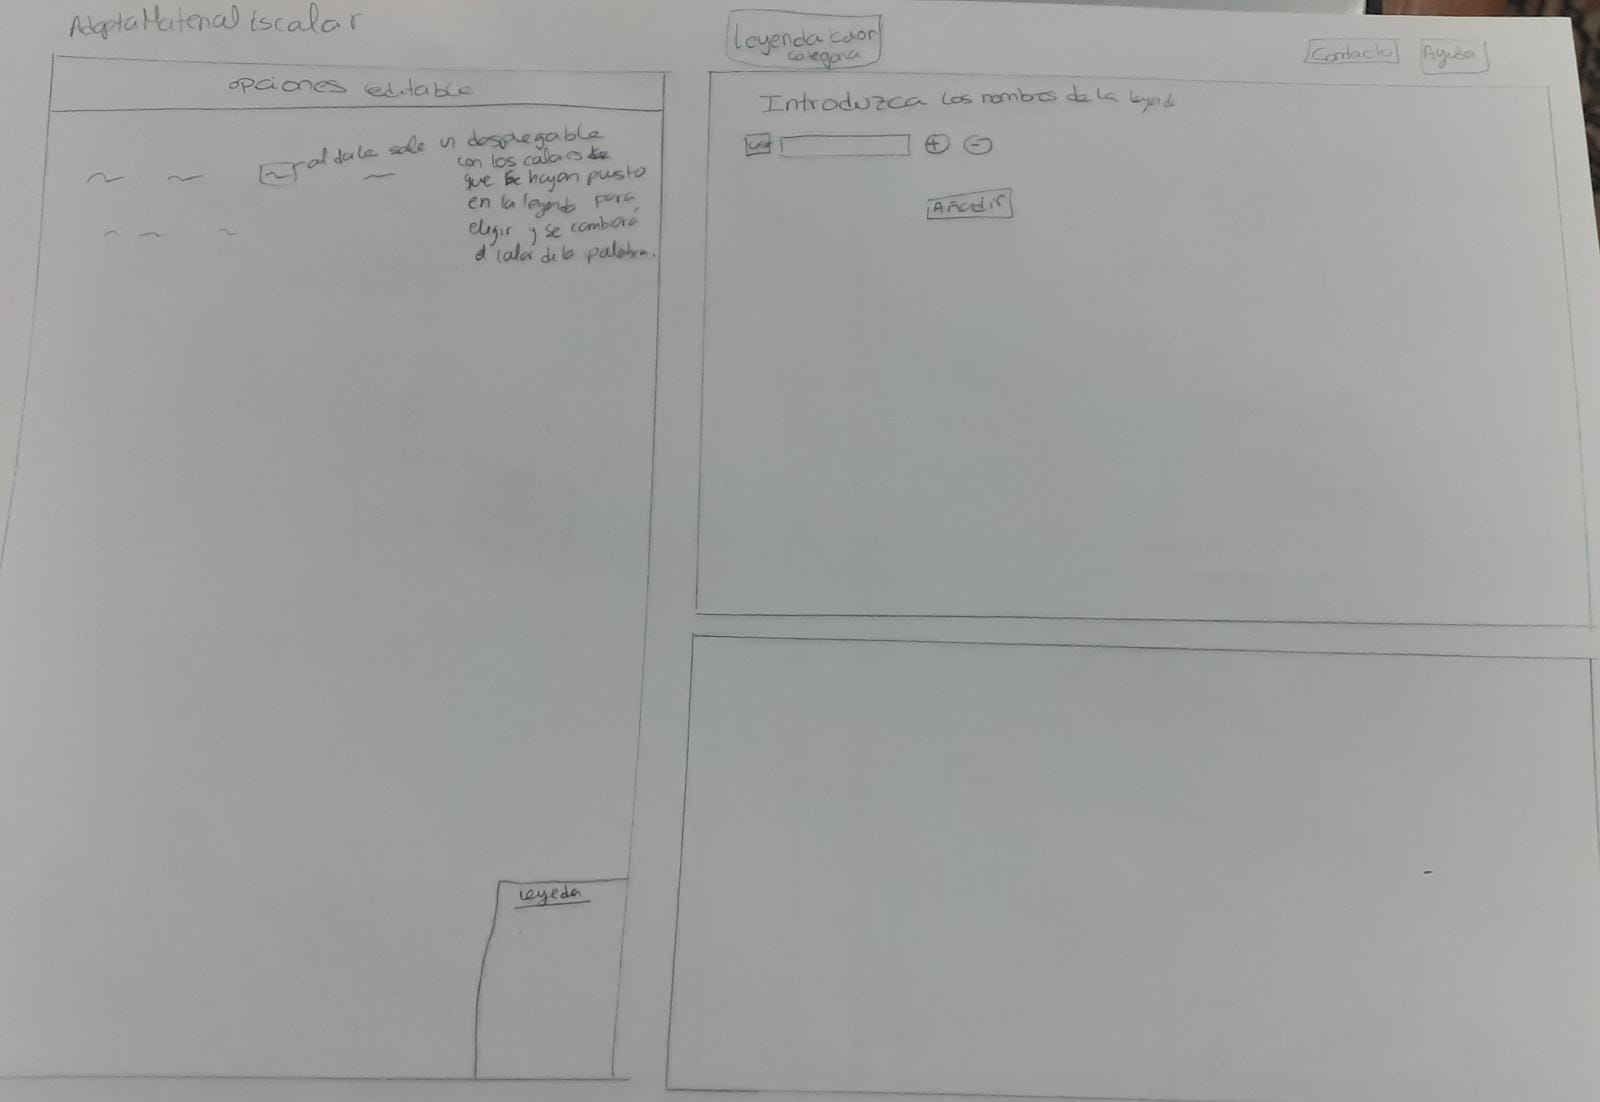
\includegraphics[width=0.7\textwidth]{Diseño/Dunia/leyendaColor.jpeg}
    \caption{Diseño de leyenda de colores de Dunia.}
    \label{dunia5}
  \end{figure}

  \begin{figure}[ht!]
    \centering
    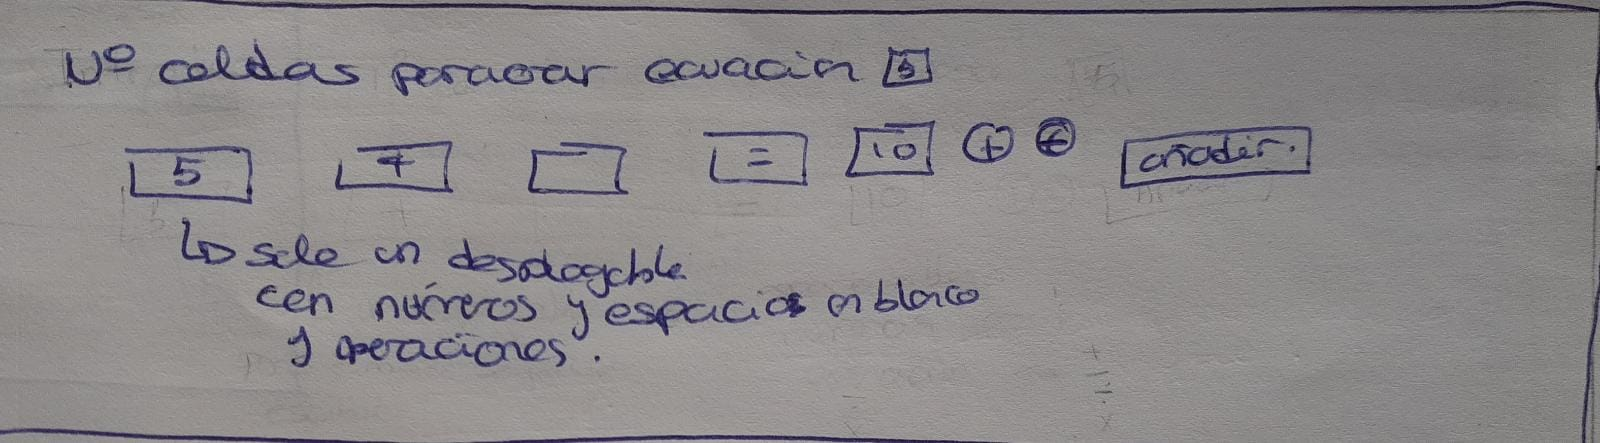
\includegraphics[width=0.7\textwidth]{Diseño/Dunia/hueco.jpeg}
    \caption{Diseño de ejercicios matemáticas de huecos de Dunia.}
    \label{dunia6}
  \end{figure}